\chapter{Subsystem: Communications} \label{chap:communications}

\begin{figure}[H]
	\centering
	\begin{subfigure}{.5\textwidth}
		\centering
		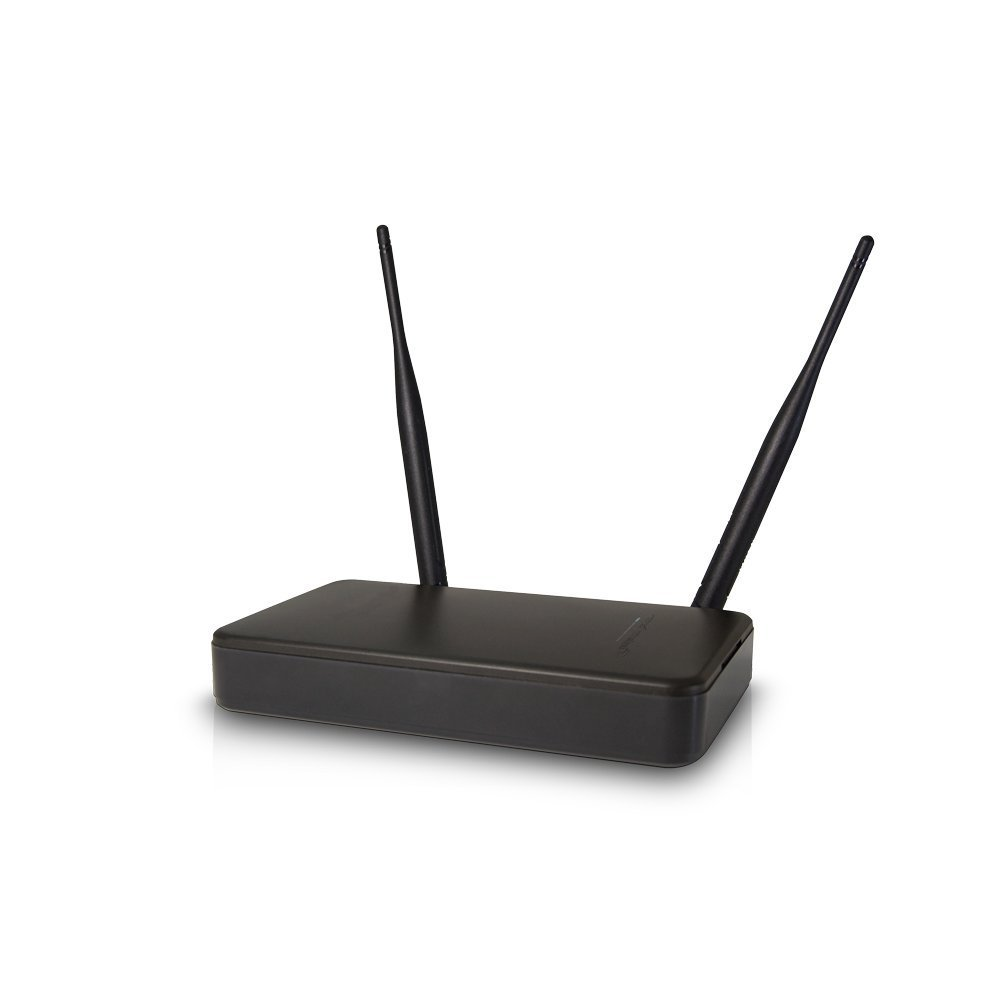
\includegraphics[width=.8\linewidth]{amped}
		\caption{Amped Wireless High Power Wifi Router}
		\label{fig:sub1}
	\end{subfigure}%
	\begin{subfigure}{.5\textwidth}
		\centering
		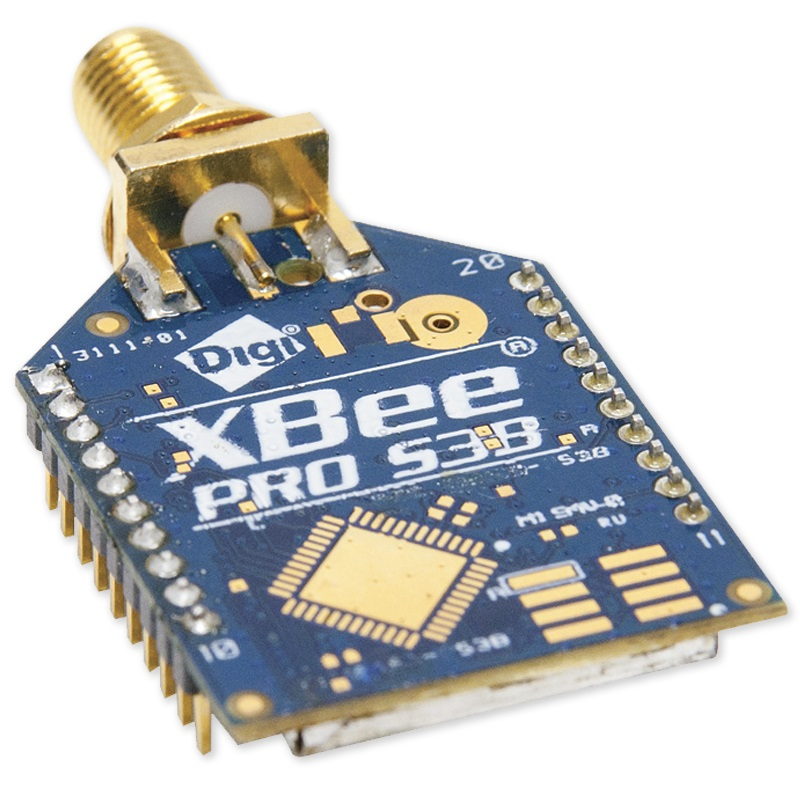
\includegraphics[width=.8\linewidth]{xbee}
		\caption{XBee PRO 900hp}
		\label{fig:sub2}
	\end{subfigure}
	\caption{Communication Subsystem}
	\label{fig:test}
\end{figure}

In order to meet our design objectives, our vehicle needs to be able to relay information back to its operator and receive commands from the operator.  In order to achieve this, we need to design a strong communication link between the vehicle and the operator.

Our current implementation uses a peer-to-peer wifi network to receive feedback from the vehicle and an XBee PRO for vehicle driving commands.  Peer-to-peer wifi networks are easy to setup and maintain and provide the high bandwidth required to transmit the camera and sensor data from the vehicle to the operators. However, the main problem with the peer-to-peer wifi network is that it has a relatively short range. The connection is not good at long distances, and the actual distance varies depending on if there are any objects in between the network nodes. For safety and reliability reasons, we chose to keep the XBee PRO communication link between the control console and rover for the driving commands. The XBee has a much lower bandwidth, but a much higher range (theoretical 28 miles, line-of-sight).

In order to meet our design requirement of 150 meters line-of-sight communication link, we chose to install a  Amped Wireless High Power Wireless-N 600mW Gigabit Router (R10000G). While the theoretical range of this device is dependent on the wifi performance of the receiving device, our field tests demonstrated an actual range of over 300 meters.

We recognize that the shortcomings of a peer-to-peer network are unacceptable and unsafe for our application. However, due to budget constraints and the technology that we had readily available to us, we decided to use the peer-to-peer wifi network anyways. This will be enough to develop a functioning prototype of the vehicle and implement all of the other functionality that we need to.

In order to create a market ready solution, future teams should look to update this subsystem and use a technology that has a greater range and reliability.